\chapter{Evaluation of radiation}\label{evaluation}
In current version of the code following types of radiation are implemented: synchrotron radiation, inverse Compton scattering, gamma-ray emission due to pion decay in free-free proton interaction and also bremsstrahlung.

Abstract class RadiationEvaluator and it's inherited classes are used for evaluation of radiation. There are derved classes for every specific type of radiation and also class RadiationSumEvaluator which allows to sum several different types of radiation. Public methods of this two classes are listed in Table \ref{radiationEvaluator}. 

General approach to evaluation of radiation is following: create radiation source, using one of the classes, described in Section \ref{sourcesSection}, or user-defined, then create object of radiation evaluator, which types are described below, and then call method evaluateFluxFromSource(const double\& photonFinalEnergy, RadiationSource* source) of this object, which evaluates energy density of the energy flux from source in units $\rm cm^{-2} s^{-1}$.

\begin{figure}[h]
	\centering
	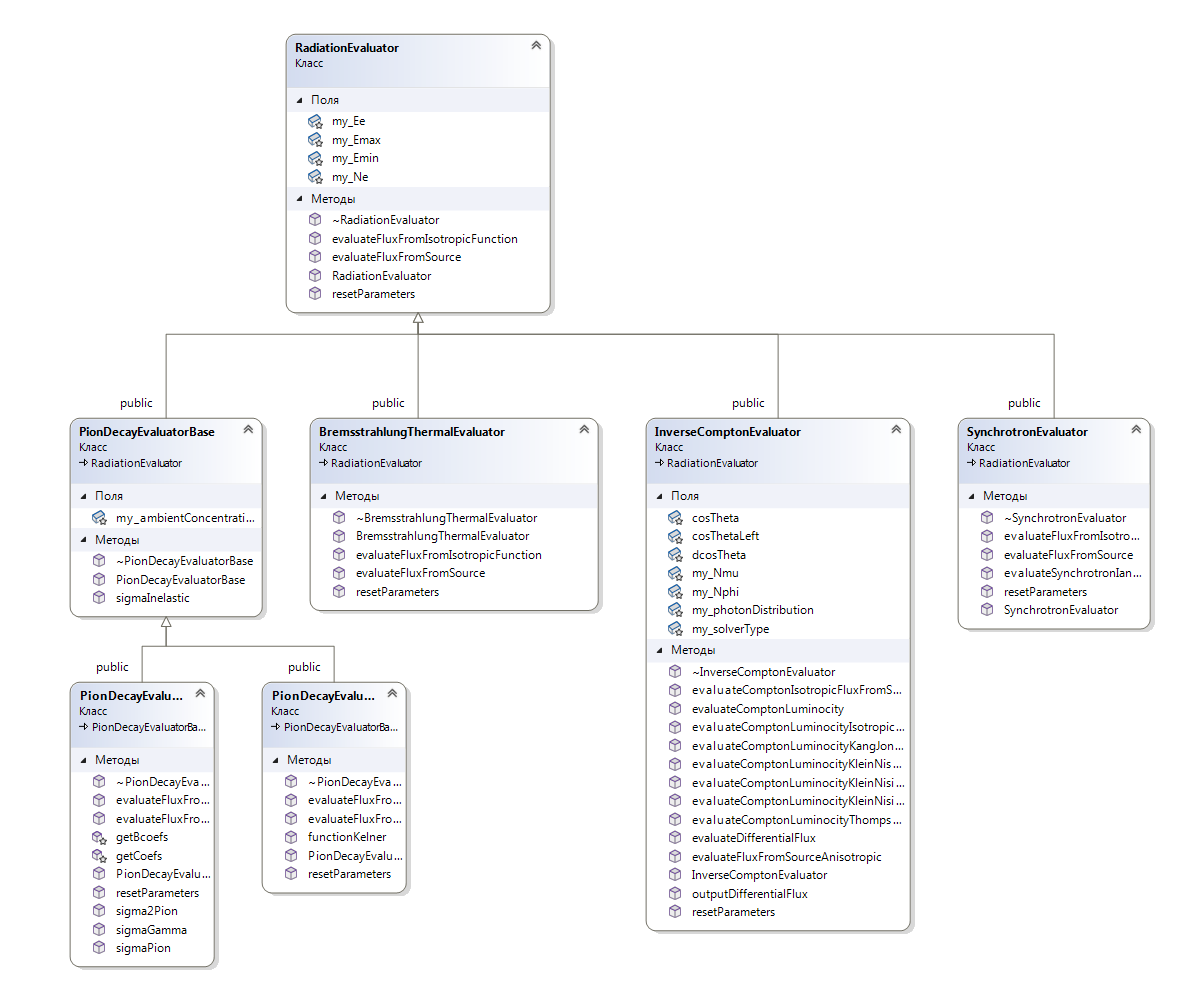
\includegraphics[width=10.5 cm]{./fig/radiationEvaluator.png} 
	\caption{class hierarchy of radiation evaluators}
	\label{radiationEvaluators}
\end{figure}

Classes for every specific type of electromagnetic radiation are described below in this chapter. Class hierarchy of radiation evaluators is shown in Figure \ref{radiationEvaluators}. Equations used for evaluation are discussed in Chapter \ref{Formulae}.

\begin{small}
	\topcaption{Public methods of RadiationEvaluator class}
	\label{radiationEvaluator}
	\begin{xtabular}{|p{0.51\textwidth}|p{0.49\textwidth}|} 
		\hline
		\textbf{RadiationEvaluator} & astract class for evaluation of radiation \\
		\hline
		virtual evaluateFluxFromSource(const double\& photonFinalEnergy, RadiationSource* source) & virtual method, returns energy density of radiation energy flux in units $\text{cm}^{-2} \text{s}^{-1}$ \\
		\hline
		virtual double evaluateFluxFromSourceAtPoint(const double\& photonFinalEnergy, RadiationSource* source, int rhoi, int phi) & virtual method, returns energy density of radiatio energy flux from given grid cell on tangent plane\\
		\hline
		double evaluateTotalFluxInEnergyRange(const double\& Ephmin, const double\& Ephmax, int Nph, RadiationSource* source) & returns integrated energy flux in the given energy range, evaluted by Nph points distributied logarithmically, in units $\text{erg} \text{cm}^{-2} \text{s}^{-1}$\\
		\hline
		virtual resetParameters( const double* parameters, const double* normalizationUnits) & virtual method, reseting parameters of the radiation evaluator. Lists of parameters are different for different types of evaluators. Method takes for input array of parameters in normalized units, and array of normalization conctants. This method for example is used for fitting modelled radiation to the observational data and optimization.\\
		\hline
		writeFluxFromSourceToFile(const char* fileName, RadiationSource* source, const double\& Ephmin, const double\& Ephmax, const int Nph) & evaluates and writes into the file energy density of radiation energy flux in given energy range with Nph points distributed logarithmically. Writes two columns of data in units $\text{erg}$  and $\text{cm}^{-2} \text{s}^{-1}$\\
		\hline
		writeImageFromSourceToFile(const char* fileName, RadiationSource* source, const double\& Ephmin, const double\& Ephmax, const int Nph) & evaluates and writes to file image - energy flux from every cell of the tangent plane in units $\text{erg} \text{cm}^{-2} \text{s}^{-1}$ integrated in given energy range with Nph points distributed logarithmically\\
		\hline
		writeImageFromSourceAtEToFile(const double\& photonFinalEnergy, const char* fileName, RadiationSource* source) & evaluates and writes to file image - energy density of radiation energy flux from every cell of the tangent plane in units $\text{cm}^{-2} \text{s}^{-1}$\\
		\hline
		\textbf{RadiationSumEvaluator} & class for sum of several types of radiation\\
		\hline
		RadiationSumEvaluator(int Ne, const double\& Emin, const double\& Emax, RadiationEvaluator* evaluator1, RadiationEvaluator* evaluator2) & constructor, creates evaluator which sums results of two given evaluators, and takes into accaunt emmiting particles in given energy range\\
		\hline
		RadiationSumEvaluator(int Ne, const double\& Emin, const double\& Emax, int Nev, RadiationEvaluator** evaluators) & constructor, creates evaluator which sums results of given array of evaluators, and takes into accaunt emmiting particles in given energy range\\
		\hline
	\end{xtabular}
\end{small}

\section{Synchrotron radiation}\label{synchrotronSection}
Class SynchrotronEvaluator is implemented for evaluation of synchrotron radiation. It uses standard approximation of continious spectrum, described in \cite{Ginzburg1975, Ghisellini} and in section \ref{synchrotronFormulaSection},  - it is valid for frequencies of emitted photons much higher than gyrofrequency of emitting particles. Also it is possible to take into account synchrotron self-absorption. Cylindrical geomtry, shown in Figure \ref{sphericalLayer} allows to integrate flux through the line of sight and take into account absorption inside the source. To create SynchrotronEvaluator object user should provide energy range of particles to be taken into account, numbers of integration points in it, and also two boolean parameters - for accounting self absorption and doppler shifting due to source matter velocity. Public methods of Synchrotron evaluator are listed in Table  \ref{SynchrotronEvaluator}. Example of evaliation of synchrotron radiation is shown in section Running simple problem.
\begin{table}[h]
	\begin{center}
	\begin{small}
	\caption{Public methods of SynchrotronEvaluator}
	\label{SynchrotronEvaluator}
	\begin{tabularx}{\textwidth}{|X|X|} 
		\hline
		\textbf{SynchrotronEvaluator} & class for evaluation synchrotron radiation\\
		\hline
		SynchrotronEvaluator( int Ne, double Emin, double Emax, bool selfAbsorption = true, bool doppler = false) & constructor, creates evaluator with given energy range of particles taken into account and parameters corresponding to self-absorption and doppler effect\\
		\hline
		evaluateSynchrotronIandA(const double\& photonFinalFrequency, const double\& photonFinalTheta, const double\& photonFinalPhi, const double\& B, const double\& sinhi, const double\& concentration, MassiveParticleIsotropicDistribution* electronDistribution, double\& I, double\& A) & evaluates emissivity per unit volume and absorption coefficient for photon of given energy and direction in given magnetic field and number density and distribution of emitting particles\\
		\hline
	\end{tabularx}
\end{small}
\end{center}
\end{table}
\section{Inverse Compton scattering}
Class InverseComptonEvaluator is implemented for evaluation of radiation produced in inverce compton scattering. Also it has one derived class InverseComptonEvaluatorWithSource. The difference between them is that in the first one distribution of seed photons is constant inside the source, and in the second one photons number density is change proportionaly inverse square of the distance to the source of seed photons.

There are four different algorithmes of evaluation IC radiation that can be used by InverseComptonEvaluator, their formulae are described in section \ref{ComptonFormulaeSection}. They are listed by enum-type ComptonSolverType, having following values:

\begin{itemize}
	\item ISOTROPIC\_THOMSON - simple model of scattering in thomson regime with power-law distribution of electrons and thermal distribution of seed photons, as described in \cite{Ginzburg1975} ch 17, p. 466.
	\item ANISOTROPIC\_KLEIN\_NISHINA - model computing radiation directly by integrating Klein-Nishina cros-section as described in \cite{KleinNishina, Dubus} and in section \ref{comptonFormulaSection}. With this model is possible to evaluate radiation produced by anisotropic distributions of initial particles
	\item ISOTROPIC\_KLEIN\_NISHINA - model similar to the previous, it uses integration of Klein-Nishina cross-section, but isotropy of distributions of initial particles is assumed, and it allows to reduce number of integrations through the azimuthal angle
	\item ISOTROPIC\_JONES - model, using analytical integration through the all angular variables, in case of isotropic distributions of initial particles. It is described in \cite{JonesCompton, BykovUvarov2000} and in section??
\end{itemize}

To create object of InverseComptobEvaluator type user needs to provide energy range of particles taken into account and nimber of points to integrate through it, number of points through the polar and azimutal angle, distribution function of seed photons and algorithm of computation the radiation. Public methods of InverseComptonEvaluator and InverseComptonEvaluatorWithSource are listed in Table \ref{InverseComptonEvaluator}.
\begin{small}
	\topcaption{Public methods of inverse compton scattering evaluators}
	\label{InverseComptonEvaluator}
	\begin{xtabular}{|p{0.5\textwidth}|p{0.5\textwidth}|} 
		\hline
		\textbf{InverseComptonEvaluator} & class for evaluation radiation from inverse compton scattering\\
		\hline
		InverseComptonEvaluator( int Ne, int Nmu, int Nphi, double Emin, double Emax, PhotonDistribution* photonDistribution, ComptonSolverType solverType) & constructor, creates evaluator with given energy range of particles taken into account, numbers of integration points throught the energy and angular variables, distribution function of seed photons and method of computation the radiation\\
		\hline
		evaluateFluxFromSourceAnisotropic( const double\& photonFinalEnergy, const double\& photonFinalTheta, const double\& photonFinalPhi, PhotonDistribution* photonDistribution, RadiationSource* source) & returns energy density of radiation energy flux created by given seed photons distribution and source containing scattering particles in given direction\\
		\hline
		evaluateTotalFluxInEnergyRangeAnisotropic( const double\& Ephmin, const double\& Ephmax, const double\& photonFinalTheta, const double\& photonFinalPhi, int Nph, PhotonDistribution* photonDistribution, RadiationSource* source, ComptonSolverType solverType) & returns total energy flux of radiation created by given seed photons distribution and source containing scattering particles in given direction integrated in given energy range through Nph point distributed logarithmically.\\
		\hline
		\textbf{InverseComptonEvaluatorWithSource} & class for evaluation radiation from inverce comton scattering takin into account dependency of photons number density on distance to the source of photons\\
		\hline
		InverseComptonEvaluatorWithSource(int Ne, int Nmu, int Nphi, double Emin, double Emax, double Ephmin, double Ephmax, PhotonDistribution* photonDistribution, ComptonSolverType solverType, const double\& sourceR, const double\& sourceZ, const double\& sourcePhi) & constructor, creates evaluator with given energy range of particles taken into account, numbers of integration points throught the energy and angular variables, distribution function of seed photons with number density corresponding to the origin of coordinates, method of computation the radiation and coordinates of the source of seed photons\\
		\hline
	\end{xtabular}
\end{small}

Example of the evaluation of radiation produced by Inverse Compton scattering is shown in the function  evaluateComtonWithPowerLawDistribution() in the file examples.cpp. In this function X-ray radiation from Fast Blue Optical Transient CSS161010 is evaluated. Electrons distribution is assumed power-law as in paper \cite{Coppejans2020} and seed photons are taken from mean galactic photon field \cite{Mathis1983}.

At first let define main parameters of the source - it's size, distance to observer, electrons number density and magnetic field. Magnetic field doesn't matter for inverse compton scattering, so assume it equal to zero. Also we define numbers of grid points for integration through the energy and angular variables

\begin{lstlisting}[language=c++]
	double electronConcentration = 150;
	double sinTheta = 1.0;
	double rmax = 1.3E17;
	double B = 0.0;
	double distance = 150*1E6*parsec;
	
	double Emin = me_c2;
	double Emax = 10000 * me_c2;
	int Ne = 200;
	int Nmu = 20;
	int Nphi = 4;
\end{lstlisting}

Then we create distribution of seed photons, using static method of class MultiPlankDistribution getGalacticField wich returns mean galactic photon distribution. And also we create electron power-law distribution with spectral index 3.5

\begin{lstlisting}[language=c++]
	PhotonIsotropicDistribution* photonDistribution = 
	    PhotonMultiPlankDistribution::getGalacticField();
	MassiveParticlePowerLawDistribution* electrons = new 
	    MassiveParticlePowerLawDistribution(massElectron, 3.5,
	    Emin, electronConcentration);
\end{lstlisting}

Then we create radiation source as homogenous disk and radiation evaluator for inverse Compton scattering. Let use following method of comutation inverse compton radiation - ISOTROPIC\_KLEIN\_NISHINA, via integration Klein-Nishina cross-section with isotropic photon and electron distributions.

\begin{lstlisting}[language=c++]
    RadiationSource* source = new SimpleFlatSource(
        electrons, B, sinTheta, rmax, rmax, distance);
	
    double Ephmin = 0.1 * 2.7 * kBoltzman;
    double Ephmax = 10 * 10000 * kBoltzman;
    InverseComptonEvaluator* comptonEvaluator = new 
        InverseComptonEvaluator(Ne, Nmu, Nphi, Emin, Emax, Ephmin, Ephmax, 
        photonDistribution, ComptonSolverType::ISOTROPIC_JONES);

\end{lstlisting}

If user don't want to use standard method to writing radiation in to the file, in case of one need result in some other units - electron-volts for energy and write energy density flux in units 
$E F(E)$ - $\text{erg}~\text{cm}^{-2}\text{s}^{-1}$, user should write result to file manually. Let create grid for energy of radiated photons
\begin{lstlisting}[language=c++]
    int Nnu = 100;
    double* E = new double[Nnu];
    double* F = new double[Nnu];

    double EphFinalmin = 0.01 * kBoltzman * 2.725;
    double EphFinalmax = 2 * Emax;
    double factor = pow(EphFinalmax / EphFinalmin, 1.0 / (Nnu - 1));
    E[0] = EphFinalmin;
    F[0] = 0;
    for (int i = 1; i < Nnu; ++i) {
        E[i] = E[i - 1] * factor;
        F[i] = 0;
    }
\end{lstlisting}
and then compute energy density fluxes for this energies
\begin{lstlisting}[language=c++]
	for (int i = 0; i < Nnu; ++i) {
		F[i] = comptonEvaluator->evaluateFluxFromSource(
		    E[i], source);
	}
\end{lstlisting}
and wrtie them to file transforming to the prefered units
\begin{lstlisting}[language=c++]
	FILE* output_ev_EFE = fopen("output.dat", "w");
	
	for (int i = 0; i < Nnu; ++i) {
		fprintf(output_ev_EFE, "%g %g\n",
		    E[i] / (1.6E-12), E[i] * F[i]);
	}

	fclose(output_ev_EFE);
\end{lstlisting}
Spectrum of radiation, obtained with this code is shown in Figure \ref{compton}
\begin{figure}[h]
	\centering
	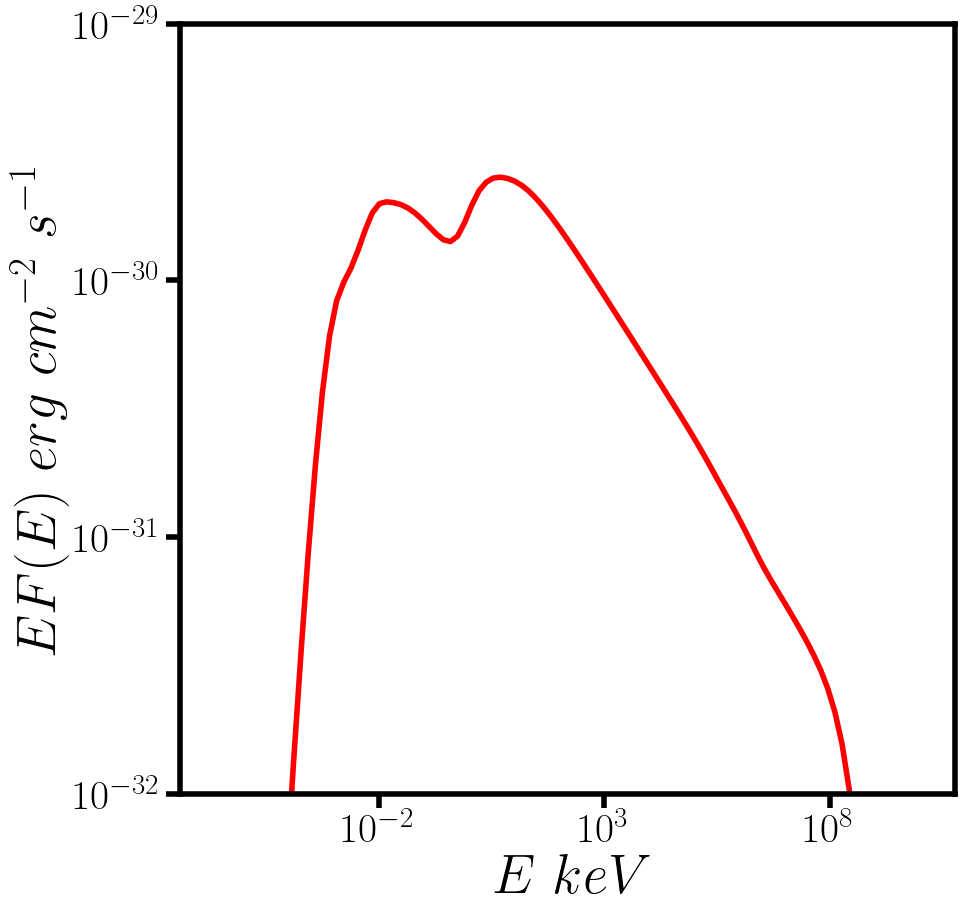
\includegraphics[width=12.5 cm]{./fig_en/compton.png} 
	\caption{Energy density flux of inverse compton radiation}
	\label{compton}
\end{figure}

\section{Pion decay}

For evaluation of gamma-radiation, produced in proton-proton inelastic collision due to pion decay, abstract class PionDecayEvaluatorBase is implemented. Also there are two derived class for different methods of computation: PionDecayEvaluatorKelner, in wich cross-section of gamma-photon remission considered a fraction of cross-section of inelastic p-p interaction as it is described in paper \cite{Kelner}, and PionDecayEvaluator in which more accurate evaluation of cross-section at low energy is used, see \cite{Kafexhiu}. Formulae are described in details in section \ref{PionFormulaeSection}. In both models it is assumed, that high energy protons with isotropic distribution are scattered on cold protons of ambient medium, and time of energy losses of fast protons due to p-p scattering is mush larger than time of particle confinment in the source, so each proton can be scattered at most one time.

To create object of pion decay evaluator user should provide energy range of particles to be taken into account, number of integration points in it and number density of ambient protons. Public methods of class PionEvaluatorBase and derived classes are listed in Table \ref{pionDecay}

		\begin{small}
			\topcaption{Public methods of class PionEvaluatorBase and inherited classes}
			\label{pionDecay}
			\begin{xtabular}{|p{0.5\textwidth}|p{0.5\textwidth}|}  
				\hline
				\textbf{PionDecayEvaluatorBase} & abstract class for evaluation gamma radiation due to pion decay\\
				\hline
				sigmaInelastic(const double\& energy) & returns cross-section of inelastic scattering moving proton on the resting in the lab frame. NOTE! method takes kinetic energy of moving proton\\
				\hline
				\textbf{PionDecayEvaluatorKelner} &
				class for evaluation gamma radiation assuming cross-section of emission is fraction of inelastic cross-section as it is described in \cite{Kelner}\\
				\hline
				PionDecayEvaluatorKelner(int Ne, double Emin, double Emax, const double\& ambientConcentration) & constructor, creates evaluator with given range of protons energy taken into account, number of integration grid points in it and number density of ambient protons \\
				\hline
				\textbf{PionDecayEvaluator} & class for evaluation gamma radiation with method described in \cite{Kafexhiu}\\
				\hline
				PionDecayEvaluator(int Ne, double Emin, double Emax, const double\& ambientConcentration) & constructor, creates evaluator with given range of protons energy taken into account, number of integration grid points in it and number density of ambient protons\\
				\hline
				sigmaGamma(const double\& photonEnergy, const double\& protonEnergy) & returns cross-section of emission of gamma photon with given energy by scattering of proton with given kinetic energy.
		        NOTE! method takes kinetic energy of moving proton\\
				\hline
			\end{xtabular}
		\end{small}
	
Example of evaluation of gamma radiation, produced by pion decay is shown in the function evaluatePionDecay() in the file examples.cpp. In this example gamma radiation from Cygnus Сocoon is evaluated. Protons are considered accelerated on the system of secondary shock as it is described in \cite{BykovKalyashova2022}. In this paper it is shown, that accelerated protons distribution is power-law with break at energy 2.2 TeV. Spectral index at low energies is 2.1 and 2.64 at high. Size of the emitting region is taken equal to the size of  Sygnus Cocoon Superbubble - 55 pc.

As usual, let define general parameters of the source - number density, it's size and distance to it and magnetic field which can be set to zero in this example. Energu range of protons is from 0.01 GeV to 10 TeV, and the energy of break of the spectrum is 2.2 TeV
\begin{lstlisting}[language=c++]
	double protonConcentration = 150;
	double rmax = 55 * parsec;
	double B = 0;
	double sinTheta = 1.0;

	double distance = 1400 * parsec;
	double Emin = massProton*speed_of_light2 + 0.01E9 * 1.6E-12;
	double Emax = 1E13 * 1.6E-12;
	double Etrans = 2.2E12 * 1.6E-12;
\end{lstlisting}
After that let create protons distribution and radiation source
\begin{lstlisting}[language=c++]
	MassiveParticleBrokenPowerLawDistribution* protons = new 
		MassiveParticleBrokenPowerLawDistribution(
		massProton, 2.1, 2.64, Emin, Etrans, protonConcentration);
	RadiationSource* source = new SimpleFlatSource(
		protons, B, sinTheta, rmax, rmax, distance);
\end{lstlisting}
Then one should create radiation evaluator. It is necessary to provide number density of ambient protons for it
\begin{lstlisting}[language=c++]
double protonAmbientConcentration = 20;
PionDecayEvaluator* pionDecayEvaluator = new PionDecayEvaluator(
	200, Emin, Emax, protonAmbientConcentration);
\end{lstlisting}
Let create energy grid for radiated gamma photons, which will be used for manual output of radiation spectrum
\begin{lstlisting}[language=c++]
    int Nnu = 200;
    double* E = new double[Nnu];
    double* F = new double[Nnu];
    double Ephmin = 0.01 * Emin;
    double Ephmax = 1E16 * 1.6E-12;
    double factor = pow(Ephmax / Ephmin, 1.0 / (Nnu -  1));
    E[0] = Ephmin;
    F[0] = 0;
    for (int i = 1; i < Nnu; ++i) {
	    E[i] = E[i - 1] * factor;
    	F[i] = 0;
    }
\end{lstlisting}
and then we can evaluate radiation energy density flux and write it into the file in preffred units
\begin{lstlisting}[language=c++]
	for (int i = 0; i < Nnu; ++i) {
		F[i] = pionDecayEvaluator->evaluateFluxFromSource(
		    E[i], source);
	}	
	FILE* output_ev_dNdE = fopen("outputPionE.dat", "w");
	for (int i = 0; i < Nnu; ++i) {
		double nu = E[i] / hplank;
		fprintf(output_ev_dNdE, "%g %g\n",
		    E[i] / (1.6E-12), F[i] / E[i]);
	}
	fclose(output_ev_dNdE);
\end{lstlisting}
Spectrum of radiation from Cygnus Cocoon, obtained with this code, and observational data by Fermi LAT, ARGO and HAWC \cite{Ackermann2011, Bartoli2014, Abeysekara2021} are shown in Figure \ref{pion}
\begin{figure}
	\centering
	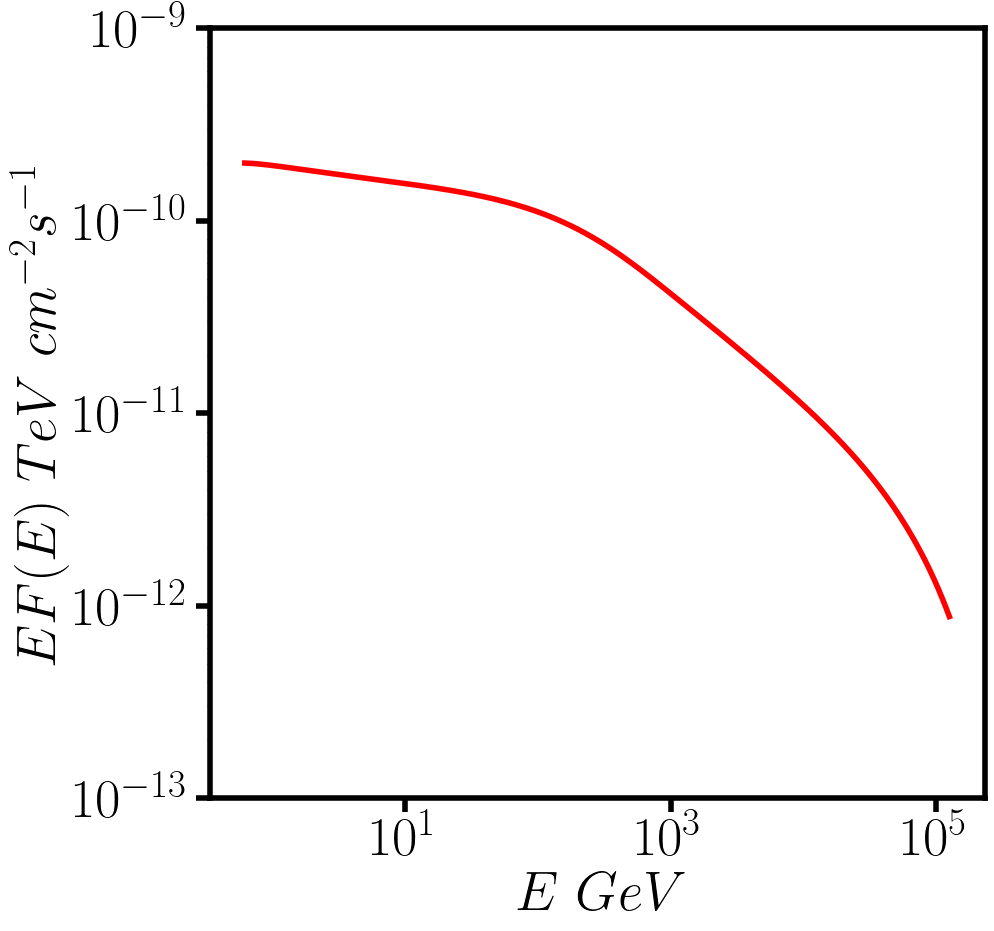
\includegraphics[width=12.5 cm]{./fig/pion.png} 
	\caption{Modeled energy flux energy density from Cygnus Cocoon and observational data}
	\label{pion}
\end{figure}

\section{Bremsstrahlung}

For evaluation of bremsstrahlung radiation, produced by electron-electron and electron-proton collisions, two classes inherited from RadiationEvaluator are implemented. BremsstrahlungThermalEvaluator uses simple analytical model, described in \cite{Rybicki}, for case with thermal distribution of particles. This class should be use for debug and calibration of the second one - BremsstrahlungEvaluator. This class uses more general approach, which can be applied for any isotropic distribution of emitting electrons. For electron-ion cross section Bethe-Heitler formula is used \cite{BetheHeitler}, which is described in detail in \cite{JauchRohrlich}. Electron-electron scattering is computed with formulae provided by \cite{Baring1999}. Formulaes are described in section \ref{BremsstrahlungFormulaeSection} and public methods of this classes are listed in Table \ref{bremsstrahlung}

\begin{small}
\topcaption{Public methods of classes BremsstrahlungThermalEvaluator and BremsstrahlungEvaluator}
	\label{bremsstrahlung}
	\begin{xtabular}{|p{0.5\textwidth}|p{0.5\textwidth}|}  
		\hline
		\textbf{BremsstrahlungThermalEvaluator} & class for evaluation bremsstrahlung radiation from plasma with thermal distribution\\
		\hline
		BremsstrahlungThermalEvaluator() & default constructor\\
		\hline
		\textbf{BremsstrahlungEvaluator} & class for evaluation bremsstrahlung radiation from plasma with isotropic distribution of emitting electrons\\
		\hline
		BremsstrahlungEvaluator( int Ne, const double\& Emin, const double\& Emax) & constructor, creates evaluator with given range of electrons energy taken into account and number of integration points in it. With this constructor density of ions is assumed zero, and only electron-electron collisions would be computed.\\
		\hline
		BremsstrahlungEvaluator( int Ne, const double\& Emin, const double\& Emax, double protonsRelativeConcentration) & constructor, creates evaluator with given range of electrons energy taken into accoun, number of integration points in it, and relative number density of protons to electrons. If it is equal to 1, number density of protons is considered equal to the number density of protons.\\
		\hline
		BremsstrahlungEvaluator( int Ne, const double\& Emin, const double\& Emax, int ionNumber, double* ionConcentrations, int* ionCharges) & constructor, creates evaluator with given range of electrons energy taken into accoun, number of integration points in it, number of types of ions, they relative number densities and charges in units of elementary charge. Note! Electro-neutrality is on user's responsibility.\\
		\hline
		double evaluateSigma( const double\& gammaE, const double\& epsilonG) & returns cross-section of emitting photon with energy $\epsilon_G$ in units $m_e c^2$ in energy range $d\epsilon_G$ by electron with Lorentz-factor $\gamma_e$, integrated by all angular variables.\\
		\hline
	\end{xtabular}
\end{small}

Example of evaluation of bremsstrahlung is shown in function  evaluateBremsstrahlung in the file examples.cpp. In this example we compare results of computations of thermal plasma radiation obtained with two bremsstrahlung evaluator classes. As always we start with defining parameters of the source. Now we also define the temperature of hot relativistic plasma.

\begin{lstlisting}[language=c++]
    double electronConcentration = 1;
    double rmax = 1.3E17;
    double B = 0;
    double temperature = 1E10;
	
    double distance = 150 * 3.08 * 1.0E24;
    double Emin = me_c2;
    double Emax = me_c2 + 100 * kBoltzman * temperature;
\end{lstlisting}

Then we create Maxwell-Juttner distribution of electrons, and radiation source as homogenous flat disk

\begin{lstlisting}[language=c++]
    MassiveParticleMaxwellJuttnerDistribution* electrons = new 
        MassiveParticleMaxwellJuttnerDistribution( 
        massElectron, temperature, electronConcentration);
    RadiationSource* source = new 
        SimpleFlatSource(electrons, 0, 0, rmax, rmax, distance);
\end{lstlisting}

Also we create two different bremsstrahlung evaluator. Number density of protons we set to be equal number density of electrons.

\begin{lstlisting}[language=c++]
    int Ne = 500;
    BremsstrahlungThermalEvaluator* bremsstrahlungEvaluator1 = new
        BremsstrahlungThermalEvaluator();
    BremsstrahlungEvaluator* bremsstrahlungEvaluator2 = new
    	BremsstrahlungEvaluator(Ne, Emin, Emax, 1.0);
\end{lstlisting}

Then as usual we create grid for frequensies of emitted photons. Minimal and maximal energy of photons depend on temperature of plasma.

\begin{lstlisting}[language=c++]
    int Nnu = 200;
    double* E = new double[Nnu];

    double Ephmin = 0.001 * kBoltzman * temperature;
    double Ephmax = 100 * kBoltzman * temperature;
    double factor = pow(Ephmax / Ephmin, 1.0 / (Nnu - 1));
    E[0] = Ephmin;
    for (int i = 1; i < Nnu; ++i) {
        E[i] = E[i - 1] * factor;
    }	
\end{lstlisting}

And finally we evaluate photons energy flux with two different evaluators and write it into the file

\begin{lstlisting}[language=c++]
    FILE* output_ev_EFE = fopen("outputBremE.dat", "w");
    FILE* output_GHz_Jansky = fopen("outputBremNu.dat", "w");
    for (int i = 0; i < Nnu; ++i) {
        double nu = E[i] / hplank;
        printf("%d\n", i);
        printLog("%d\n", i);
        double F1 = bremsstrahlungEvaluator1->evaluateFluxFromSource(
            E[i], source);
        double F2 = bremsstrahlungEvaluator2->evaluateFluxFromSource(
            E[i], source);
        fprintf(output_ev_EFE, "%g %g %g\n",
            E[i] / (1.6E-12), E[i] * F1, E[i] * F2);
        fprintf(output_GHz_Jansky, "%g %g %g\n",
            nu / 1E9, 1E26 * hplank * F1, 1E26 * hplank * F2);
    }
    fclose(output_ev_EFE);
    fclose(output_GHz_Jansky);
\end{lstlisting}

Modeled energy density of energy flux is shown in Figure \ref{bremsstrahlungFigure}. In the limit of it's applicability simple analytical model provides results close to the results of more precise computations.

\begin{figure}
	\centering
	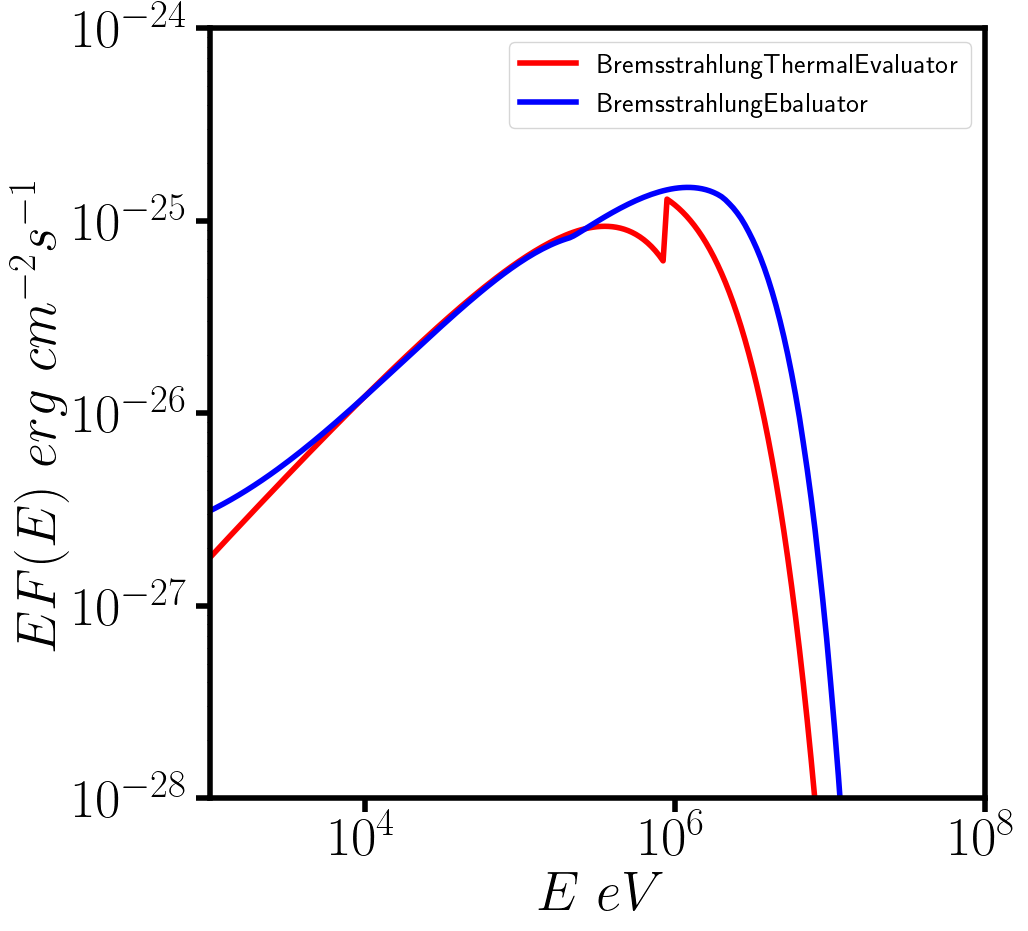
\includegraphics[width=12.5 cm]{./fig_en/bremsstrahlung.png} 
	\caption{Modeled spectrum of bremsstrahlung radiation of hot thermal plasma}
	\label{bremsstrahlungFigure}
\end{figure}
